%
\newpage
\chapter{Introducción}
  \section{Sistemas Complejos}
      Un sistema complejo es definido tipicamente como un sistema que es "más que la suma de sus partes", es decir, mientras que de forma individual los elementos del sistema pueden ser muy sencillos y fáciles de analizar, el comportamiento del sistema como un todo es altamente complejo y difícil de predecir.\cite{3}

      Un sistema complejo se encuentra formado por un número elevado de componentes elementales (autómatas), que interactúan de forma local entre ellos y con el entorno que los rodea. Son sistemas cuya evolución es muy complicada de predecir ya que aparecen comportamientos (comportamiento emergente) que es difícil de predecir considerando los parámetros iniciales.
      
      Las interacciones entre los individuos no suele ser lineal, es decir, existen proceso de retroalimentación, comunicación o inhibición en los mismos. Pueden variar su estructura con el tiempo, es decir, la creación de nuevos individuos, nuevos enlaces; como un sistema dinámico. \cite{1}
      
      Una de las premisas más grandes es la que menciona que comportamientos simples suelen dar lugar a comportamientos macroscópicos complejos, como se pudo ver al realizar el análisis de los atractores del juego de la vida de John Conway.\cite{2}

      \begin{figure}[h!]
        \centering
          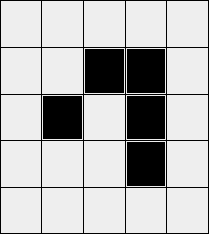
\includegraphics[scale=0.4]{./images/glider}
          \caption{Glider: Elemento del juego de la vida.} 
      \end{figure}

    \subsection{Características de los sistemas complejos}
      Una de las principales características de los sistemas complejos es la convivencia y relación entre los elementos con el sistema y consigo mismos, por ejemplo, un agente o automáta que tiene una visibilidad limitada de sus sitema. Un claro ejemplo es la vecindad de Moore utilizada mucho en el análisis de automatas celulares.\cite{4}
      
      Otro factor a tomar en cuenta como principio de los sistemas complejos es que todas la unidades (automatas o elementos) son considerados como trabajos en paralelo, es decir, podrían ser vistos como computadoras independientes y cuyo procesamiento no depende uno del otro.

      Los sistemas complejos como un todo muestran fenómenos emergentes, fuera de las interacciones entre las unidades simples, emerge un comportamiento complejo, patrones o inteligencia. Es bien sabido que los ejemplos existen, por ejemplo las colonias de hormigas, patrones de migración, terremotos, copos de nieve, etc.

      Finalmente, se pueden identificar tres aspectos de los sistemas complejos, es importante mencionar que puede ser una diversa mezcla de éstas y no todos los sistemas complejos las tienen.

      \textbf{No lineal}: Este aspecto de los sistemas complejos suele ser referido como ``el efecto mariposa'', acuñado al matemático y meteorólogo Edward Norton Lorenz, pionero en el estudio de la teoría del caos. Se le llama ``no lineal'' por qué no hay una relación donde un ligero cambio pueda ser visualizado dada una cierta función, es decir, pequeños cambios implican nuevos resultados. Los sistemas no lineales son un superconjunto de los sistemas caóticos.

      \textbf{Competición y cooperación}: Una de las cosas que suelen ser visualizadas en un sistema complejo es la presencia de competición y cooperación entre los elementos. Esto puede ser visualizado durante el análisis de ciertos procesos naturales, por ejemplo, el sistema inmunológico; donde se puede ver a los glóbulos blancos (Linfocítos) distribuirse, comunicarse y cooperar para la erradicación de posibles invasores al sistema. No todos los sistemas complejos pueden mostrar ese tipo de comportamiento, por ejemplo, un análisis climatológico.

      \textbf{Estocásticos}: Esta propiedad nos habla del azar o bien de la facultad de tomar o no cierta acción o decisión. El comportamiento de un sistema complejo puede ser reflejado mediante procesos aleatorios dentro de sus movimientos o interacciones dentro del sistema y con sus vecinos.

      \textbf{Retroalimentación}: Los sistemas complejos suelen contener retroalimentación donde la salida de un sistema se convierte en la entrada del mismo generando resultados distintos. Esta es una de las principales causas de que los sistemas complejos no sean lineales.\cite{3} \cite{5}

      Un elemento clave de los sistemas complejos son los autómatas celulares, éstos surgen en la década de 1940 con John Von Neumann, que intentaba modelar una máquina que fuera capaz de autoreplicarse, llegando así a un modelo matemático de dicha máquina con reglas complicadas sobre una red rectangular.

      Inicialmente fueron interpretados como conjunto de células que crecían, reproducían y morían a medida que pasaba el tiempo. A esta similitud con el crecimiento de las células se le debe su nombre.

      Un autómata celular es un modelo matemático para un sistema dinámico, compuesto por un conjunto de celdas o células que adquieren distintos estados o valores. Los elementos base de los autómatas celulares se listan a continuación:
      \begin{itemize}
        \item{\textbf{Arreglo Regular}: Ya sea en un plano de dos dimensiones o un espacio n-dimensional, este es el espacio de evoluciones, y cada división homogénea de arreglo es llamado célula.}
        \item{\textbf{Conjunto de estados}: Es finito y cada elemento o célula del arreglo toma un valor de éste conjunto de estados. También se le denomina alfabeto y puede ser expresado en valores o colores.}
        \item{\textbf{Configuración inicial}: Consiste en asignar un estado a cada una de las células del espacio de evolución inicial del sistema.}
        \item{\textbf{Vecindades}: Define el conjunto contiguo de células y posición relativa respecto a cada una de ellas. A cada vecindad diferente le coresponde un elemento del conjunto de estados.}
        \item{\textbf{Función Local}: Es la regla de evolución que determina el comportamiento del autómata celular. Se conforma de una célula central y sus vecindades. Define como debe cambiar de estado cada célula dependiendo los estados anteriores de sus vecindades.}
        \item{\textbf{Limites}: Puede ser abierta, reflectora, periódica o sin frontera.}
      \end{itemize}
    Es importante destacar la complejidad que se logra con un autómata celular. De acuerdo a la dimensión en la que se genere tendrá un número potencial de vecinos, generando una gran cantidad de combinaciones y posibles estados.

    \begin{figure}[h!]
      \centering
        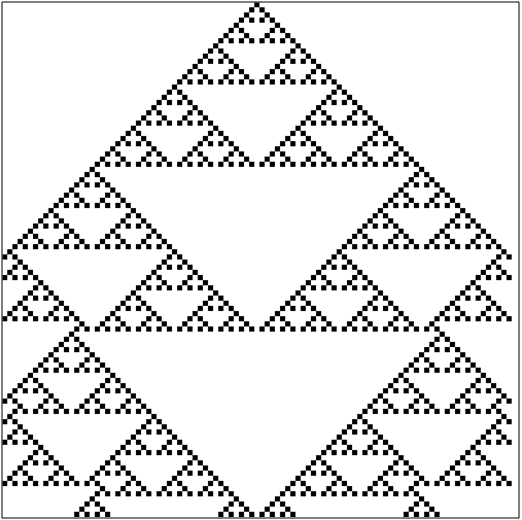
\includegraphics[scale=0.4]{./images/CellularAutomata}
        \caption{Patrón generado por un autómata celular.} 
    \end{figure}

    Los autómatas celulares han sido usados en distintas disciplinas, por ejemplo:
      \begin{itemize}
        \item{\textbf{Física}: Aplicación en la simulación de la dinámica de fluidos.}
        \item{\textbf{Biología}: Para proceso de modelización de ecosistemas.}
        \item{\textbf{Química}: Para el estudio cinético de las reacciones y simulación del crecimiento de cristales.}
        \item{\textbf{Computación}: Construcción de modelos para el procesamiento de información en paralelo. Arquitecturas de computadoras basadas en principios y materiales biológicos. \cite{10}}
      \end{itemize}
    Stephen Wolfram comenzó a trabajar en autómatas celulares a mediados de 1981. Sus investigaciones fueron inicialmente impulsadas por un interés en sistemas de modelado, como las redes neuronales. Wolfram define cuatro clases en las que los autómatas celulares, considerando la complejidad de éstos. La clasificación e identificación que propone Wolfram es la siguiente:
      \begin{itemize}
        \item{\textbf{Clase I}: Casi todos los patrones evolucionan rápidamente en un estado estable y homogéneo. Cualquier aletoriedad en el patrón inicial desaparece.}
        \item{\textbf{Clase II}: Casi todos los patrones iniciales evolucionan rápidamente hacia estructuras estables u oscilantes. Parte de la aleatoridad del patrón inicial puede peramencer pero sólo algunos restos. Los cambios locales en el patrón inicial tienden a permanecer locales.}
        \item{\textbf{Clase III}: Casi todos los patrones iniciales evolucionan de forma pseudo-aleatoria o caótica: Las estructuras estables que aparecen son destruidas rápidamente por el ruido circundante. Los cambios locales en el patrón tienden a propagarse indefinidamente.}
        \item{\textbf{Clase IV}: Casi todos los patrones iniciales evolucionan en las estructuras que interactúan de manera compleja e interesante, con la formación de las estructuras locales que son capaces de sobrevivir por largos periodos de tiempo. Podría ser el caso de que apareciesen estructuras estables u oscilantes, pero el momento de pasos necesarios para llegar a ese estado puede ser muy grande, incluso cuando el patrón inicial es relativamente simple.}
      \end{itemize}
    Estas definiciones son de carácter cualitativo, y hay cierto margen de interpretación. Según Wolfram ``Con casi cualquier esquema de clasificación general, hay casos en los que, inevitablemente, se asignan a una clase por definición y otra clase por otra definición, y lo mismo ocurre con los autómatas celulares: hay veces que las reglas muestran algunas características de una clase y otras de otra clase''.\cite{11}